\section{Máquinas de Pilha Abstratas}

\begin{frame}[fragile]{Máquinas de Pilha Abstratas}

    \begin{itemize}
        \item A interface de vanguarda do compilador produz uma representação intermediária do programa fonte, que será usada pela interface de retaguarda para
            produzir o programa alvo
        \pause

        \item Uma possível forma para a representação intermediária é a máquina de pilha abstrata
        \pause

        \item Uma máquina de pilha abstrata possui memórias separadas para dados e instruções, e todas as operações aritméticas são realizadas sobre os valores
            em uma pilha
        \pause

        \item As instruções são divididas em três classes: aritmética inteira, manipulação de pilha e fluxo de controle
        \pause

        \item O ponteiro $pc$ indica qual é a próxima instrução a ser executada
    \end{itemize}

\end{frame}

\begin{frame}[fragile]{Instruções aritméticas}

    \begin{itemize}
        \item  A máquina de pilha abstrata precisa implementar cada operador da linguagem intermediária
        \pause

        \item Operações elementares, como adição e subtração, são suportadas diretamente
        \pause

        \item Operações mais sofisticadas devem ser implementadas como uma sequência de instruções da máquina
        \pause

        \item A título de simplificação, assuma que existe uma instrução para cada operação aritmética
        \pause

        \item O código de uma máquina de pilha abstrata para uma expressão simula a avaliação de um representação posfixa, usando uma pilha
        \pause

        \item A avaliação segue da esquerda para a direita, empilhando os operandos
        \pause

        \item  Quando um operador é encontrado, seus operandos são extraídos da pilha
        (do último para o primeiro), a operação é realizada e o resultado é inserido no topo da pilha
    \end{itemize}

\end{frame}

\begin{frame}[fragile]{Comportamento do analisador preditivo não-recursivo para a cadeia ``$\textbf{id}\code{apl}{+}\textbf{id}\code{apl}{×}\textbf{id}$''}

    \begin{tikzpicture}
        \node[opacity=0] at (12, 0) { . };
        \node[opacity=0] at (12, 7) { . };

        \node at (2.5, 0.5) { \texttt{Pilha} };

        \draw[very thick] (1.5, 1) to (3.5, 1);

        \draw[thick] (2, 1) rectangle (3, 2);
        \node at (2.5, 1.5) { \texttt{\$} };

        \draw[thick] (2, 2) rectangle (3, 3);
        \node at (2.5, 2.5) { $E$ };

        \node[anchor=west] at (5, 5) { \texttt{Entrada} };

        \node[anchor=west] at (6, 4) { \textbf{id} \code{apl}{+} \textbf{id} \code{apl}{×} \textbf{id} \texttt{\$} };

        \node[anchor=west] at (10, 5) { \texttt{Saída} };

%        \node[anchor=west] at (11, 4) { $E'\to \code{apl}{+}TE'$ };
    \end{tikzpicture}

\end{frame}

\begin{frame}[fragile]{Comportamento do analisador preditivo não-recursivo para a cadeia ``$\textbf{id}\code{apl}{+}\textbf{id}\code{apl}{×}\textbf{id}$''}

    \begin{tikzpicture}
        \node[opacity=0] at (12, 0) { . };
        \node[opacity=0] at (12, 7) { . };

        \node at (2.5, 0.5) { \texttt{Pilha} };

        \draw[very thick] (1.5, 1) to (3.5, 1);

        \draw[thick] (2, 1) rectangle (3, 2);
        \node at (2.5, 1.5) { \texttt{\$} };

        \draw[thick] (2, 2) rectangle (3, 3);
        \node at (2.5, 2.5) { $E$ };

        \node[anchor=west] at (5, 5) { \texttt{Entrada} };

        \node[anchor=west] at (6, 4) { \textbf{id} \code{apl}{+} \textbf{id} \code{apl}{×} \textbf{id} \texttt{\$} };
        \draw[-latex,thick] (6.3, 3.2) to (6.3, 3.8);

        \node[anchor=west] at (10, 5) { \texttt{Saída} };

%        \node[anchor=west] at (11, 4) { $E'\to \code{apl}{+}TE'$ };
    \end{tikzpicture}

\end{frame}

\begin{frame}[fragile]{Comportamento do analisador preditivo não-recursivo para a cadeia ``$\textbf{id}\code{apl}{+}\textbf{id}\code{apl}{×}\textbf{id}$''}

    \begin{tikzpicture}
        \node[opacity=0] at (12, 0) { . };
        \node[opacity=0] at (12, 7) { . };

        \node at (2.5, 0.5) { \texttt{Pilha} };

        \draw[very thick] (1.5, 1) to (3.5, 1);

        \draw[thick] (2, 1) rectangle (3, 2);
        \node at (2.5, 1.5) { \texttt{\$} };

        \draw[thick] (2, 2) rectangle (3, 3);
        \node at (2.5, 2.5) { $E'$ };

        \draw[thick] (2, 3) rectangle (3, 4);
        \node at (2.5, 3.5) { $T$ };

        \node[anchor=west] at (5, 5) { \texttt{Entrada} };

        \node[anchor=west] at (6, 4) { \textbf{id} \code{apl}{+} \textbf{id} \code{apl}{×} \textbf{id} \texttt{\$} };
        \draw[-latex,thick] (6.3, 3.2) to (6.3, 3.8);

        \node[anchor=west] at (10, 5) { \texttt{Saída} };

        \node[anchor=west] at (11, 4) { $E\to TE'$ };
%        \node[anchor=west] at (11, 4) { $E'\to \code{apl}{+}TE'$ };
    \end{tikzpicture}

\end{frame}

\begin{frame}[fragile]{Comportamento do analisador preditivo não-recursivo para a cadeia ``$\textbf{id}\code{apl}{+}\textbf{id}\code{apl}{×}\textbf{id}$''}

    \begin{tikzpicture}
        \node[opacity=0] at (12, 0) { . };
        \node[opacity=0] at (12, 7) { . };

        \node at (2.5, 0.5) { \texttt{Pilha} };

        \draw[very thick] (1.5, 1) to (3.5, 1);

        \draw[thick] (2, 1) rectangle (3, 2);
        \node at (2.5, 1.5) { \texttt{\$} };

        \draw[thick] (2, 2) rectangle (3, 3);
        \node at (2.5, 2.5) { $E'$ };

        \draw[thick] (2, 3) rectangle (3, 4);
        \node at (2.5, 3.5) { $T'$ };

        \draw[thick] (2, 4) rectangle (3, 5);
        \node at (2.5, 4.5) { $F$ };

        \node[anchor=west] at (5, 5) { \texttt{Entrada} };

        \node[anchor=west] at (6, 4) { \textbf{id} \code{apl}{+} \textbf{id} \code{apl}{×} \textbf{id} \texttt{\$} };
        \draw[-latex,thick] (6.3, 3.2) to (6.3, 3.8);

        \node[anchor=west] at (10, 5) { \texttt{Saída} };

        \node[anchor=west] at (11, 4) { $T\to FT'$ };
%        \node[anchor=west] at (11, 4) { $E'\to \code{apl}{+}TE'$ };
    \end{tikzpicture}

\end{frame}

\begin{frame}[fragile]{Comportamento do analisador preditivo não-recursivo para a cadeia ``$\textbf{id}\code{apl}{+}\textbf{id}\code{apl}{×}\textbf{id}$''}

    \begin{tikzpicture}
        \node[opacity=0] at (12, 0) { . };
        \node[opacity=0] at (12, 7) { . };

        \node at (2.5, 0.5) { \texttt{Pilha} };

        \draw[very thick] (1.5, 1) to (3.5, 1);

        \draw[thick] (2, 1) rectangle (3, 2);
        \node at (2.5, 1.5) { \texttt{\$} };

        \draw[thick] (2, 2) rectangle (3, 3);
        \node at (2.5, 2.5) { $E'$ };

        \draw[thick] (2, 3) rectangle (3, 4);
        \node at (2.5, 3.5) { $T'$ };

        \draw[thick] (2, 4) rectangle (3, 5);
        \node at (2.5, 4.5) { \textbf{id} };

        \node[anchor=west] at (5, 5) { \texttt{Entrada} };

        \node[anchor=west] at (6, 4) { \textbf{id} \code{apl}{+} \textbf{id} \code{apl}{×} \textbf{id} \texttt{\$} };
        \draw[-latex,thick] (6.3, 3.2) to (6.3, 3.8);

        \node[anchor=west] at (10, 5) { \texttt{Saída} };

        \node[anchor=west] at (11, 4) { $F\to \textbf{id}$ };
%        \node[anchor=west] at (11, 4) { $E'\to \code{apl}{+}TE'$ };
    \end{tikzpicture}

\end{frame}

\begin{frame}[fragile]{Comportamento do analisador preditivo não-recursivo para a cadeia ``$\textbf{id}\code{apl}{+}\textbf{id}\code{apl}{×}\textbf{id}$''}

    \begin{tikzpicture}
        \node[opacity=0] at (12, 0) { . };
        \node[opacity=0] at (12, 7) { . };

        \node at (2.5, 0.5) { \texttt{Pilha} };

        \draw[very thick] (1.5, 1) to (3.5, 1);

        \draw[thick] (2, 1) rectangle (3, 2);
        \node at (2.5, 1.5) { \texttt{\$} };

        \draw[thick] (2, 2) rectangle (3, 3);
        \node at (2.5, 2.5) { $E'$ };

        \draw[thick] (2, 3) rectangle (3, 4);
        \node at (2.5, 3.5) { $T'$ };

%        \draw[thick] (2, 4) rectangle (3, 5);
%        \node at (2.5, 4.5) { \textbf{id} };

        \node[anchor=west] at (5, 5) { \texttt{Entrada} };

        \node[anchor=west] at (6, 4) { \textbf{id} \code{apl}{+} \textbf{id} \code{apl}{×} \textbf{id} \texttt{\$} };
        \draw[-latex,thick] (6.675, 3.2) to (6.675, 3.8);

        \node[anchor=west] at (10, 5) { \texttt{Saída} };

%        \node[anchor=west] at (11, 4) { $F\to \textbf{id}$ };
%        \node[anchor=west] at (11, 4) { $E'\to \code{apl}{+}TE'$ };
    \end{tikzpicture}

\end{frame}

\begin{frame}[fragile]{Comportamento do analisador preditivo não-recursivo para a cadeia ``$\textbf{id}\code{apl}{+}\textbf{id}\code{apl}{×}\textbf{id}$''}

    \begin{tikzpicture}
        \node[opacity=0] at (12, 0) { . };
        \node[opacity=0] at (12, 7) { . };

        \node at (2.5, 0.5) { \texttt{Pilha} };

        \draw[very thick] (1.5, 1) to (3.5, 1);

        \draw[thick] (2, 1) rectangle (3, 2);
        \node at (2.5, 1.5) { \texttt{\$} };

        \draw[thick] (2, 2) rectangle (3, 3);
        \node at (2.5, 2.5) { $E'$ };

%        \draw[thick] (2, 3) rectangle (3, 4);
%        \node at (2.5, 3.5) { $T'$ };

%        \draw[thick] (2, 4) rectangle (3, 5);
%        \node at (2.5, 4.5) { \textbf{id} };

        \node[anchor=west] at (5, 5) { \texttt{Entrada} };

        \node[anchor=west] at (6, 4) { \textbf{id} \code{apl}{+} \textbf{id} \code{apl}{×} \textbf{id} \texttt{\$} };
        \draw[-latex,thick] (6.675, 3.2) to (6.675, 3.8);

        \node[anchor=west] at (10, 5) { \texttt{Saída} };

        \node[anchor=west] at (11, 4) { $T'\to \code{apl}{∊}$ };
%        \node[anchor=west] at (11, 4) { $E'\to \code{apl}{+}TE'$ };
    \end{tikzpicture}

\end{frame}

\begin{frame}[fragile]{Comportamento do analisador preditivo não-recursivo para a cadeia ``$\textbf{id}\code{apl}{+}\textbf{id}\code{apl}{×}\textbf{id}$''}

    \begin{tikzpicture}
        \node[opacity=0] at (12, 0) { . };
        \node[opacity=0] at (12, 7) { . };

        \node at (2.5, 0.5) { \texttt{Pilha} };

        \draw[very thick] (1.5, 1) to (3.5, 1);

        \draw[thick] (2, 1) rectangle (3, 2);
        \node at (2.5, 1.5) { \texttt{\$} };

        \draw[thick] (2, 2) rectangle (3, 3);
        \node at (2.5, 2.5) { $E'$ };

        \draw[thick] (2, 3) rectangle (3, 4);
        \node at (2.5, 3.5) { $T$ };

        \draw[thick] (2, 4) rectangle (3, 5);
        \node at (2.5, 4.5) { \code{apl}{+} };

        \node[anchor=west] at (5, 5) { \texttt{Entrada} };

        \node[anchor=west] at (6, 4) { \textbf{id} \code{apl}{+} \textbf{id} \code{apl}{×} \textbf{id} \texttt{\$} };
        \draw[-latex,thick] (6.675, 3.2) to (6.675, 3.8);

        \node[anchor=west] at (10, 5) { \texttt{Saída} };

        \node[anchor=west] at (11, 4) { $E'\to \code{apl}{+}TE'$ };
    \end{tikzpicture}

\end{frame}

\begin{frame}[fragile]{Comportamento do analisador preditivo não-recursivo para a cadeia ``$\textbf{id}\code{apl}{+}\textbf{id}\code{apl}{×}\textbf{id}$''}

    \begin{tikzpicture}
        \node[opacity=0] at (12, 0) { . };
        \node[opacity=0] at (12, 7) { . };

        \node at (2.5, 0.5) { \texttt{Pilha} };

        \draw[very thick] (1.5, 1) to (3.5, 1);

        \draw[thick] (2, 1) rectangle (3, 2);
        \node at (2.5, 1.5) { \texttt{\$} };

        \draw[thick] (2, 2) rectangle (3, 3);
        \node at (2.5, 2.5) { $E'$ };

        \draw[thick] (2, 3) rectangle (3, 4);
        \node at (2.5, 3.5) { $T$ };

%        \draw[thick] (2, 4) rectangle (3, 5);
%        \node at (2.5, 4.5) { \code{apl}{+} };

        \node[anchor=west] at (5, 5) { \texttt{Entrada} };

        \node[anchor=west] at (6, 4) { \textbf{id} \code{apl}{+} \textbf{id} \code{apl}{×} \textbf{id} \texttt{\$} };
        \draw[-latex,thick] (7.05, 3.2) to (7.05, 3.8);

        \node[anchor=west] at (10, 5) { \texttt{Saída} };

%        \node[anchor=west] at (11, 4) { $E'\to \code{apl}{+}TE'$ };
    \end{tikzpicture}

\end{frame}

\begin{frame}[fragile]{Comportamento do analisador preditivo não-recursivo para a cadeia ``$\textbf{id}\code{apl}{+}\textbf{id}\code{apl}{×}\textbf{id}$''}

    \begin{tikzpicture}
        \node[opacity=0] at (12, 0) { . };
        \node[opacity=0] at (12, 7) { . };

        \node at (2.5, 0.5) { \texttt{Pilha} };

        \draw[very thick] (1.5, 1) to (3.5, 1);

        \draw[thick] (2, 1) rectangle (3, 2);
        \node at (2.5, 1.5) { \texttt{\$} };

        \draw[thick] (2, 2) rectangle (3, 3);
        \node at (2.5, 2.5) { $E'$ };

        \draw[thick] (2, 3) rectangle (3, 4);
        \node at (2.5, 3.5) { $T'$ };

        \draw[thick] (2, 4) rectangle (3, 5);
        \node at (2.5, 4.5) { $F$ };

        \node[anchor=west] at (5, 5) { \texttt{Entrada} };

        \node[anchor=west] at (6, 4) { \textbf{id} \code{apl}{+} \textbf{id} \code{apl}{×} \textbf{id} \texttt{\$} };
        \draw[-latex,thick] (7.05, 3.2) to (7.05, 3.8);

        \node[anchor=west] at (10, 5) { \texttt{Saída} };

        \node[anchor=west] at (11, 4) { $T\to FT'$ };
%        \node[anchor=west] at (11, 4) { $E'\to \code{apl}{+}TE'$ };
    \end{tikzpicture}

\end{frame}

\begin{frame}[fragile]{Comportamento do analisador preditivo não-recursivo para a cadeia ``$\textbf{id}\code{apl}{+}\textbf{id}\code{apl}{×}\textbf{id}$''}

    \begin{tikzpicture}
        \node[opacity=0] at (12, 0) { . };
        \node[opacity=0] at (12, 7) { . };

        \node at (2.5, 0.5) { \texttt{Pilha} };

        \draw[very thick] (1.5, 1) to (3.5, 1);

        \draw[thick] (2, 1) rectangle (3, 2);
        \node at (2.5, 1.5) { \texttt{\$} };

        \draw[thick] (2, 2) rectangle (3, 3);
        \node at (2.5, 2.5) { $E'$ };

        \draw[thick] (2, 3) rectangle (3, 4);
        \node at (2.5, 3.5) { $T'$ };

        \draw[thick] (2, 4) rectangle (3, 5);
        \node at (2.5, 4.5) { \textbf{id} };

        \node[anchor=west] at (5, 5) { \texttt{Entrada} };

        \node[anchor=west] at (6, 4) { \textbf{id} \code{apl}{+} \textbf{id} \code{apl}{×} \textbf{id} \texttt{\$} };
        \draw[-latex,thick] (7.05, 3.2) to (7.05, 3.8);

        \node[anchor=west] at (10, 5) { \texttt{Saída} };

        \node[anchor=west] at (11, 4) { $F\to \textbf{id}$ };
%        \node[anchor=west] at (11, 4) { $E'\to \code{apl}{+}TE'$ };
    \end{tikzpicture}

\end{frame}

\begin{frame}[fragile]{Comportamento do analisador preditivo não-recursivo para a cadeia ``$\textbf{id}\code{apl}{+}\textbf{id}\code{apl}{×}\textbf{id}$''}

    \begin{tikzpicture}
        \node[opacity=0] at (12, 0) { . };
        \node[opacity=0] at (12, 7) { . };

        \node at (2.5, 0.5) { \texttt{Pilha} };

        \draw[very thick] (1.5, 1) to (3.5, 1);

        \draw[thick] (2, 1) rectangle (3, 2);
        \node at (2.5, 1.5) { \texttt{\$} };

        \draw[thick] (2, 2) rectangle (3, 3);
        \node at (2.5, 2.5) { $E'$ };

        \draw[thick] (2, 3) rectangle (3, 4);
        \node at (2.5, 3.5) { $T'$ };

%        \draw[thick] (2, 4) rectangle (3, 5);
%        \node at (2.5, 4.5) { \textbf{id} };

        \node[anchor=west] at (5, 5) { \texttt{Entrada} };

        \node[anchor=west] at (6, 4) { \textbf{id} \code{apl}{+} \textbf{id} \code{apl}{×} \textbf{id} \texttt{\$} };
        \draw[-latex,thick] (7.45, 3.2) to (7.45, 3.8);

        \node[anchor=west] at (10, 5) { \texttt{Saída} };

%        \node[anchor=west] at (11, 4) { $F\to \textbf{id}$ };
%        \node[anchor=west] at (11, 4) { $E'\to \code{apl}{+}TE'$ };
    \end{tikzpicture}

\end{frame}


\begin{frame}[fragile]{Valores-L e valores-R}

    \begin{itemize}
        \item O significado de um identificador depende da posição onde ele ocorre em uma atribuição
        \pause

        \item No lado esquerdo, o identificador se refere à localização de memória onde o valor deve ser armazenado
        \pause

        \item No lado direito, o identificador se refere ao valor armazenado na localização de memória associada ao identificador
        \pause

        \item Valor-L e valor-R se referem aos valores apropriados para os lados esquerdo e direito de uma atribuição, respectivamente
        \pause

        \item Um mesmo identificador pode ser um valor-L e um valor-R na mesma atribuição (por exemplo, o identificador \code{cpp}{x} em \code{cpp}{x = x + 1})
    \end{itemize}

\end{frame}

\begin{frame}[fragile]{Manipulação da pilha}

    Uma máquina de pilha abstrata suporta as seguintes instruções para a manipulação da pilha:
    \begin{table}
        \center 
        \begin{tabularx}{0.9\textwidth}{p{3cm}X}
            \toprule
            \textbf{Instrução} & \textbf{Significado} \\
            \midrule
            \code{cpp}{push} $v$ & empilha $v$ \\
            \code{cpp}{pop} & desempilha o valor do topo da pilha \\
            \code{cpp}{valor-r} $p$ & empilha o valor armazenado no endereço de memória $p$ \\
            \code{cpp}{valor-l} $p$ & empilha o endereço de memória $p$ \\
            \code{cpp}{:=} & o valor-R do topo da pilha é armazenado no valor-L do subtopo (elemento que está abaixo do topo) da pilha \\
            \code{cpp}{copiar} & empilha o valor do topo da pilha \\
            \bottomrule
        \end{tabularx}
    \end{table}

\end{frame}

\begin{frame}[fragile]{Tradução de expressões}

    \begin{itemize}
        \item O código para avaliar uma expressão na máquina de pilha abstrata tem uma relação direta com a notação posfixa
        \pause

        \item Por exemplo, a expressão \code{cpp}{a + b} é traduzida para o código intermediário
            \inputsyntax{cpp}{codes/soma.cpp}
        \pause

        \item As atribuições são traduzidas da seguinte maneira: o valor-L do identificador é empilhado, a expressão à direita é avaliada e o seu valor $r$ é
            atribuído ao identificador
        \pause

        \item Formalmente,
        \[
            cmd \to \mathbf{id} := expr \ \{\ cmd.t := \code{cpp}{"valor-l"}\ ||\ \mathbf{id}.lexema\ ||\ expr\ ||\ \code{cpp}{":="}\ \}
        \]
    \end{itemize}

\end{frame}

\begin{frame}[fragile]{Tradução da expressão \code{cpp}{F = 9*C/5 + 32} para máquina de pilha abstrata}
    \inputcode{cpp}{codes/c_to_f.cpp}
\end{frame}

\begin{frame}[fragile]{Fluxo de controle}

    \begin{itemize}
        \item A máquina de pilha abstrata executa as instruções sequencialmente, na ordem em que foram dadas
        \pause

        \item Há três formas de se especificar um desvio (salto) no fluxo de execução
        \pause
        \begin{enumerate}
            \item o operando da instrução fornece o endereço da localização alvo;
            \pause 

            \item o operando da instrução fornece a distância relativa (positiva ou negativa) a ser saltada
            \pause

            \item o alvo é especificado simbolicamente (a máquina deve suportar rótulos)
            \pause
        \end{enumerate}

        \item Nas duas primeiras formas, uma alternativa é especificar que o salto está no topo da pilha
        \pause

        \item A terceira forma é a mais simples de se implementar, pois não há necessidade de se recalcular os endereços caso o número de instruções seja
            modificado durante a otimização
    \end{itemize}

\end{frame}

\begin{frame}[fragile]{Instruções de fluxo de controle}

    Uma máquina de pilha abstrata suporta as seguintes instruções para o fluxo de controle:
    \begin{table}
        \center 
        \begin{tabularx}{0.9\textwidth}{p{3cm}X}
            \toprule
            \textbf{Instrução} & \textbf{Significado} \\
            \midrule
            \code{python}{rótulo} $r$ & especifica o rótulo $r$ como possível alvo de desvios; não há outros efeitos \\
            \code{python}{goto} $r$ & a próxima instrução é tomada a partir do rótulo $r$ \\
            \code{python}{gofalse} $r$ & desempilha o topo da pilha: salta para $r$ se o valor for igual a zero \\
            \code{python}{gotrue} $r$ & desempilha o topo da pilha: salta para $r$ se o valor for diferente de zero \\
            \code{python}{parar} & encerra a execução \\
            \bottomrule
        \end{tabularx}
    \end{table}

\end{frame}

\begin{frame}[fragile]{Gabaritos para tradução de condicionais e laços}

    \begin{figure}
        \centering 
        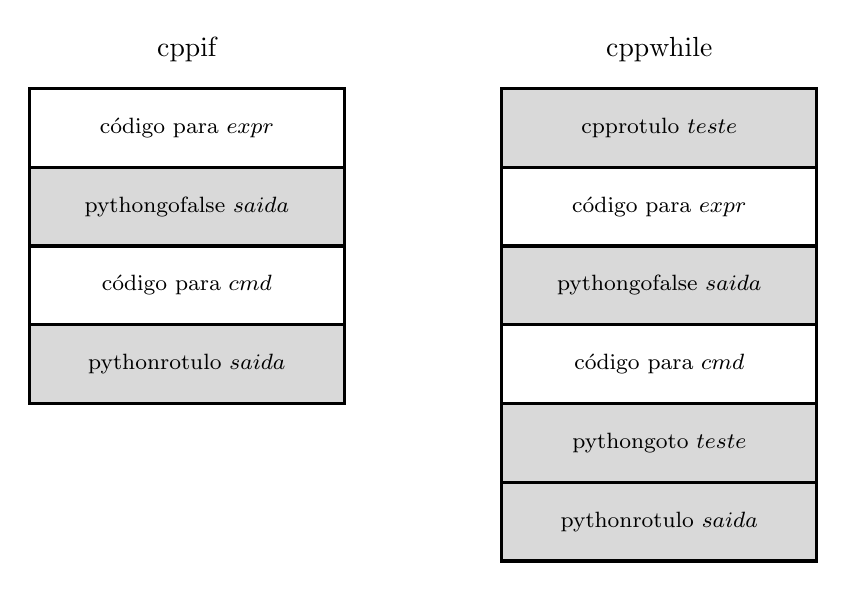
\begin{tikzpicture}
            \node at (2, 6.5) { \code{cpp}{if} };

            \draw[very thick] (0, 5) rectangle (4, 6);
            \node at (2, 5.5) { \footnotesize código para $expr$ };
            \draw[very thick,fill=gray!30] (0, 4) rectangle (4, 5);
            \node at (2, 4.5) { \footnotesize \code{python}{gofalse} $saida$ };
            \draw[very thick] (0, 3) rectangle (4, 4);
            \node at (2, 3.5) { \footnotesize código para $cmd$ };
            \draw[very thick,fill=gray!30] (0, 2) rectangle (4, 3);
            \node at (2, 2.5) { \footnotesize \code{python}{rotulo} $saida$ };

            \node at (8, 6.5) { \code{cpp}{while} };

            \draw[very thick,fill=gray!30] (6, 5) rectangle (10, 6);
            \node at (8, 5.5) { \footnotesize \code{cpp}{rotulo} $teste$ };
            \draw[very thick] (6, 4) rectangle (10, 5);
            \node at (8, 4.5) { \footnotesize código para $expr$ };
            \draw[very thick,fill=gray!30] (6, 3) rectangle (10, 4);
            \node at (8, 3.5) { \footnotesize \code{python}{gofalse} $saida$ };
            \draw[very thick] (6, 2) rectangle (10, 3);
            \node at (8, 2.5) { \footnotesize código para $cmd$ };
            \draw[very thick,fill=gray!30] (6, 1) rectangle (10, 2);
            \node at (8, 1.5) { \footnotesize \code{python}{goto} $teste$ };
            \draw[very thick,fill=gray!30] (6, 0) rectangle (10, 1);
            \node at (8, 0.5) { \footnotesize \code{python}{rotulo} $saida$ };


        \end{tikzpicture}
    \end{figure}

\end{frame}

\begin{frame}[fragile]{Unicidade dos rótulos}

    \begin{itemize}
        \item Os rótulos $saida$ e $teste$ que ilustram os gabaritos das condicionais e dos laços devem ser únicos, para evitar possíveis ambiguidades
        \pause

        \item É preciso, portanto, de uma estratégia que torne tais rótulos únicos durante a tradução
        \pause

        \item Seja $novoRotulo$ um procedimento que gera, a cada chamada, um novo rótulo único
        \pause

        \item A ação semântica associada ao comando \code{pascal}{if} assumiria a seguinte forma:
        \[
            \begin{array}{rll}
            cmd \to \code{pascal}{if}\ expr\ \code{pascal}{then}\ cmd_1 \ \{\ & saida & := novoRotulo; \\
            & cmd.t & := expr.t\ \\ & & ||\ \code{cpp}{"gofalse"}\ saida\ \\ & & ||\ cmd_1.t \\
            & & ||\ \code{cpp}{"rotulo"}\ saida\ \}
            \end{array}
        \]
    \end{itemize}

\end{frame}
